% @Author: soheilred
% @Date:   2018-10-28 01:10:54
% @Last Modified by:   soheilred
% @Last Modified time: 2018-11-07 15:30:03
\documentclass{beamer}

\let\val\undefined
\usepackage{pgf}
\usepackage{pgfplots}
\usepackage{tikz}
\usepackage{booktabs}
\usepackage{natbib}
\usepackage{framed}
\usepackage{longtable}
\usepackage{bigdelim,multirow}
\usepackage{amsmath}
\usepackage{amsthm}
\usepackage{mathtools}


\usetikzlibrary{arrows,automata,backgrounds,positioning,decorations,intersections,matrix}

% *** Styles ***
\setbeamertemplate{navigation symbols}{}
\usecolortheme{dolphin}
%\usecolortheme{rose}
\setbeamercovered{transparent}
\usefonttheme{professionalfonts}
%\usefonttheme[onlymath]{serif}

% 
\addtobeamertemplate{navigation symbols}{}{%
    \usebeamerfont{footline} %
    \usebeamercolor[fg]{footline}%
    \hspace{1em}%
    \insertframenumber/\inserttotalframenumber
}

\DeclarePairedDelimiter{\norm}{\lVert}{\rVert}
\DeclarePairedDelimiter\abs{\lvert}{\rvert}%


% \setlist[itemize,1]{label=$\times$}
% \setlist[itemize,2]{label=$\checkmark$}
% \setlist[itemize,3]{label=$\diamond$}
% \setlist[itemize,4]{label=$\bullet$}


% *** Colors ***
\newcommand{\tc}[2]{\textcolor{#1}{#2}}
\newcommand{\tcb}[1]{\tc{blue}{#1}}
\newcommand{\tcr}[1]{\tc{red}{#1}}
\newcommand{\tcg}[1]{\tc{green}{#1}}

\def\checkmark{\tikz\fill[scale=0.4](0,.35) -- (.25,0) -- (1,.7) -- (.25,.15) -- cycle;} 

\newcommand{\Ex}{\mathbb{E}}
%\newcommand{\Pr}{\mathbb{P}}
\DeclareMathOperator{\Var}{Var}
\DeclareMathOperator{\argmax}{argmax}

\definecolor{varcolor}{RGB}{132,23,49}
\newcommand{\varname}[1]{\textcolor{varcolor}{\mathsf{#1}}}

\title{Model-based Interval Estimation for MDP}
\author{Alexander L. Strehl, Micheal L. Littman \\
Journal of Computer and System Science - Elsevier\\
\textbf{IF}: 1.497}

\date{}

\begin{document}
\begin{frame}
	\maketitle

\end{frame}
%=====================================%
\begin{frame}
	\frametitle{Background}
	\begin{itemize}
		\item Exploration or exploitation? \textbf{k-armed bandit problem}
		\item Probability Approximately Correct (PAC)
		\item Confidence Intervals
		\item Model-based Interval Estimation (MBIE)
		% \item Performance metrics (mostly PAC like), but \tcr{average loss} has more \emph{online} behavior
	\end{itemize}

\end{frame}
%=====================================%

%=====================================%
\begin{frame}
	\frametitle{k-armed bandit}
	\begin{center}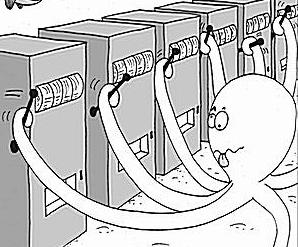
\includegraphics[width=.4\linewidth]{multiarmedbandit.jpg}\end{center}	
	\begin{itemize}
		\item k arms, one choice at a time, a payoff, drawn from an unknown distribution with mean \tcr{$\mu_i$} and variance
		\item \textbf{optimal long term}: always select the arm with highest known mean.
		$$ \argmax_i \{\mu_i\}$$
		\item Any problems?
	\end{itemize}

\end{frame}
%=====================================%

%=====================================%
\begin{frame}
	\frametitle{k-armed bandit}
	\begin{itemize}
		\item You don't get the chance to \textbf{explore} other machines
		\item Or, you don't get the chance to \textbf{exploit} what it was learned
		\item You just waste money to learn!
		\item Solution: Interval Estimation (IE)
	\end{itemize}

\end{frame}
%=====================================%

%=====================================%
\begin{frame}
	\frametitle{Interval Estimation}
	\begin{itemize}
		\item In each \textbf{trial}, construct \textbf{confidence interval} for the mean of the payoff distribution for each \textbf{arm}
		$$ [\hat{\mu_i} - \epsilon_i, \hat{\mu_i} + \epsilon_i] $$
		\item If the confidence interval is loose, the mean payoff may not be near optimal, we need to gain more information
		\item What is missing? \tcr{$\epsilon$}
		\item Model-based Interval Estimation (MBIE) is based on PAC optimality.
	\end{itemize}

\end{frame}
%=====================================%

%=====================================%
\begin{frame}
	\frametitle{What is PAC?}
	\begin{itemize}
		\item Probability Approximately Correct
		\item First developed for supervised learning classification problems
		\item Set of observations instances $X$
		\item Set of hypothesis $H$
		\begin{itemize}
			\item class of linear functions
			\item class of polynomials
			\item class of radial basis functions
		\end{itemize}
		\item Set of concepts $C$
		\item Training set $\{ (x_i, y_i) \}_i^m = \{ (x_i, \tcr{c(x_i)}) \}_i^m$
		$$y = c(x), \quad c \in C $$
		$$\hat{y} = h(x), \quad h \in H $$

		% There are some hypothesis that are consistent with the training set. If you apply that hypothesis on your training set, the training error would be zero. But, we don't know about the test set. There are a couple of these hypothesis. And there are some others that the training error is not zero (they are not consistent with the training set). The set of hypothesis that is consistent with the training set is called version space (there is no error).

		% Theorem: If hypothesis set H is finite, and D is a sequence of m>1 independent random examples of some target concept c, then for any $\epsilon \in [0,1]$, the probability that VS contains a hypothesis with error greater than $\epsilon$ is less than $$ |H|e^{-\epsilon m } $$.

		% I want to put a bound on the true error (test error). How bad my classifier would be for a classifier that classifies all of my training set correctly. What is the chance of having a classifier that do bad on test and do very good on train set.
		\item What is the probability that a classifier (with $\epsilon$ chance of misclassification), classifies correctly (Err is test error)
		$$ Pr(Err > \epsilon) < |H|e^{\epsilon m} $$ 

		% a classifier that has a true error of $\epsilon$, where has zero training error. This classifier classifies a point with $1 - \epsilon$ probability correctly. 
		$|H|e^{-\epsilon m} < \delta \rightarrow$
		$m \geq 1/\epsilon (ln|H| + ln(1/\delta))$
	\end{itemize}
	\footnotetext{Watch this! It's good! \url{https://www.youtube.com/watch?v=qOMOYM0WCzU&t=1181s}}
\end{frame}
%=====================================%

% %=====================================%
% \begin{frame}
% 	\frametitle{Average Loss?}
% 	\begin{itemize}
% 		\item 
% 	\end{itemize}
% \end{frame}
% %=====================================%

%=====================================%
\begin{frame}
	\frametitle{MBIE}
	\begin{itemize}
		\item Definitions
		\begin{itemize}
			\item occupancy count $n(s,a)$
			\item next-state count $n(s,a,s')$
			\item model size limit $m$
		\end{itemize}
		\item Reward Confidence Interval
		\begin{itemize}
			\item immediate reward from taking action a from state s: \newline r[1], r[2], ... r[n(s,a)]
			\item empirical mean reward
			$$ \hat{R}(s,a) = \frac{1}{n(s,a)} \sum_{i=1}^{n(s,a)} r[i] $$
			\item confidence interval
			$$ CI(R) = (\hat{R}(s,a)-\epsilon_{n(s,a)}^R , \hat{R}(s,a)+\epsilon_{n(s,a)}^R) $$
			$$ \epsilon_{n(s,a)}^R = \sqrt{\frac{2/\delta_r}{2.n(s,a)}} $$
		
		\end{itemize}
	\end{itemize}
\end{frame}
%=====================================%

%=====================================%
\begin{frame}
	\frametitle{How PAC is applied to MDPs?}
	\begin{itemize}
		\item ???
	\end{itemize}
\end{frame}
%=====================================%

%=====================================%
\begin{frame}
	\frametitle{MBIE}
	\begin{itemize}
		\item Transition Confidence Interval
		$$ \hat{T}(s'|s,a) = \frac{n(s,a,s')}{n(s,a)} $$
		$$ \epsilon_{n(s,a)}^T = \sqrt{\frac{2(ln(2^{|S|}) - 2) - ln(\delta_T)}{m}} $$
		\item from Hoeffiding bounds, with probability at least $1-\delta$, $R$ and $T$ are in the confidence interval
	\end{itemize}
\end{frame}
%=====================================%

%=====================================%
\begin{frame}
	\frametitle{MBIE}
	\begin{itemize}
		\item Value iteration with confidence interval:
		\begin{multline}
		  Q'(s,a) = \max_{\tilde{R}(s,a) \in CI(R)} \tilde{R}(s,a) + \\ \max_{\tilde{T}(s,a) \in CI(T)} \gamma \sum_{s'} \tilde{T}(s'|s,a) \max_{a'} Q(s',a')
		\end{multline}

		\item MBIE-EB solves
		\begin{multline}
		  Q'(s,a) = \tilde{R}(s,a) +\gamma \sum_{s'} \tilde{T}(s'|s,a) \max_{a'} \tilde{Q}(s',a') + \frac{\beta}{\sqrt{n(s,a)}}
		\end{multline}
	\end{itemize}
	\footnotetext{item page 5, difference between MBIE and MBIE-EB}

	

\end{frame}
%=====================================%

% %=====================================%
% \begin{frame}
% 	\frametitle{Background}
% 	\begin{itemize}
% 		\item 
% 	\end{itemize}
% \end{frame}
% %=====================================%


%=====================================%

\begin{frame}
	\begin{center}
		\Huge Thank You!
	\end{center}
\end{frame}
%=====================================%

% \begin{frame}
	% \frametitle{Background}
% 	\begin{itemize}
% 		\item 
% 	\end{itemize}
% \end{frame}


\end{document}
